\input{common/latex-teach-common/page-setup}
\input{common/latex-teach-common/packages}
\input{common/latex-teach-common/macros}

\renewcommand{\title}[2]{
    \documenttitle{Com3529}{Software Testing \& Analysis}{#1}{#2}
}

% URLs
\newcommand{\coderepourl}{\url{https://github.com/philmcminn/com3529-code}\xspace}

% Code snippets
\newcommand{\code}[1]{\mbox{\tt #1}\xspace}

% README file
\newcommand{\readmefile}{{\tt README.md}\xspace}

% Directories
\newcommand{\lecturesdirectory}{\code{lectures}\xspace}
\newcommand{\practicalsdirectory}{\code{practicals}\xspace}

% Packages
\newcommand{\lecturespackage}{\code{uk.ac.shef.com3529.lectures}}
\newcommand{\lecturesexecutionpackage}{\code{uk.ac.shef.com3529.lectures.execution}}
\newcommand{\practicalspackage}{\code{uk.ac.shef.com3529.practicals}}

% Classes
\newcommand{\calendarclass}{\code{Calendar}}
\newcommand{\randomlytesttriangleclass}{\code{RandomlyTestTriangle}}
\newcommand{\signutilsclass}{\code{SignUtils}}
\newcommand{\spacedefenderclass}{\code{SpaceDefender}}
\newcommand{\stringutilsbuggyoneclass}{\code{StringUtilsBuggy1}}
\newcommand{\triangleclass}{\code{Triangle}}
\newcommand{\weekoneclass}{\code{Week1}}
\newcommand{\teststringutilsbuggyoneclass}{\code{TestStringUtilsBuggy1}}
\newcommand{\testweekoneclass}{\code{TestWeek1}}


% Methods
\newcommand{\classifymethod}{\code{classify}}
\newcommand{\daysbetweentwodatesmethod}{\code{daysBetweenTwoDates}}
\newcommand{\instrumentedclassifymethod}{\code{instrumentedClassify}}
\newcommand{\randomlytestclassifymethod}{\code{randomlyTestClassify}}
\newcommand{\signmethod}{\code{sign}}

% for logic tables
\newcommand{\LTTrue}{T}
\newcommand{\LTFalse}{F}


\booltrue{shownotes}


\begin{document}

\title{Automatic Test Case Generation}{5.2 Search-Based Testing}

\section{Introduction}

\note{Video}{First slide}

One disadvantage of Random Testing, or Fuzzing, is that if certain sets of
inputs needed for a test case, or to violate some property, occupy a very small
fraction of the overall input domain, they won't be found very quickly. And if
the overall input domain is very large, or even infinite, they may not be found
at all.

\note{Video}{Next slide}

What if we could somehow {\it guide} the process to the right areas of the input
domain? Well, this is what Search-Based Testing aims to do. 

\note{Video}{Click for next point}

Search-Based Testing treats the input domain of a program as a {\it search
space}. 

\note{Video}{Click for next point}

Using heuristics, Search-Based Testing can find inputs for test cases that for
Random Testing cannot. Viewed through this lens, Random Testing tries to
(unsuccessfully) tackle ``needle in a haystack'' search problems --- without
some hints as to where the needle is (i.e., the required test data), it will
never find it.

\section{Fitness Functions}
In order to provide guidance to the required test case, Search-Based Testing
needs a {\it fitness function}. The fitness function takes an input to the
program and returns a {fitness value} indicating ``how good'' the input is to
the one that is actually needed. If the fitness function is being {\it
minimised}, the closer the value to zero, the better the input is. On the other
hand, if the fitness function is being maximised, the higher the value (usually
relative to some ceiling, maximum fitness value), the better the input is.
%
Note that the fitness function doesn't need to know {\it what} the required
input is (that would be tantamount to having solved the problem already!), just
how exactly some candidate input ``measures up'' to the one that we want.

It's easier to explain with an example. Let's return to the classify triangle
problem again. Recall that Random Testing could not easily find inputs where the
three sides are equal, i.e. {\tt side1 == side2} and {\tt side2 == side3}.

Essentially with this particular test case generation problem, Random Testing
does not ``know'' if it's getting close to the input needed to trigger the
problematic branch or not. For example, it may get equal numbers for two of the
sides, but narrowly miss out on the third. This input would be judged in exactly
the same way as one where the three sides were very far apart in value.
Search-Based Testing, on the other hand, seeks to retain ``close'' inputs and
develop them further to try to seek to execute the goal of the test case. The
fitness function it would seek to minimise in this case would be:

\begin{center}
$\mathit{fitness} = |$ {\tt side1} $-$ {\tt side2} $| + |$ {\tt side2} $-$ {\tt
side3} $|$
\end{center}

That is, absolute difference of {\tt side1} compared with {\tt side2} added to
the same calculation with {\tt side2} and {\tt side3}.

Notice how the result of this equation is closer to zero the closer the values
of the three sides are to being the same as one another, as shown by the
examples in the following table:

\begin{center}
    \begin{tabular}{rrrr}
        \toprule 
        {\tt side1} & {\tt side2} & {\tt side3} & $\mathit{fitness}$ \\
        \midrule
        10 & 20 & 30 & 20 \\
        10 & 15 & 20 & 10 \\
        10 & 12 & 14 & 4  \\
        10 & 11 & 12 & 2  \\
        10 & 10 & 10 & 0  \\
        \bottomrule
    \end{tabular}
\end{center}

We can see this visually for making {\tt side1} and {\tt side2} equal (i.e., the
first addend of the equation) by plotting the fitness values:

We call the surface of fitness values like this the fitness ``landscape''. 

\begin{center}
    \vspace{-1em}
    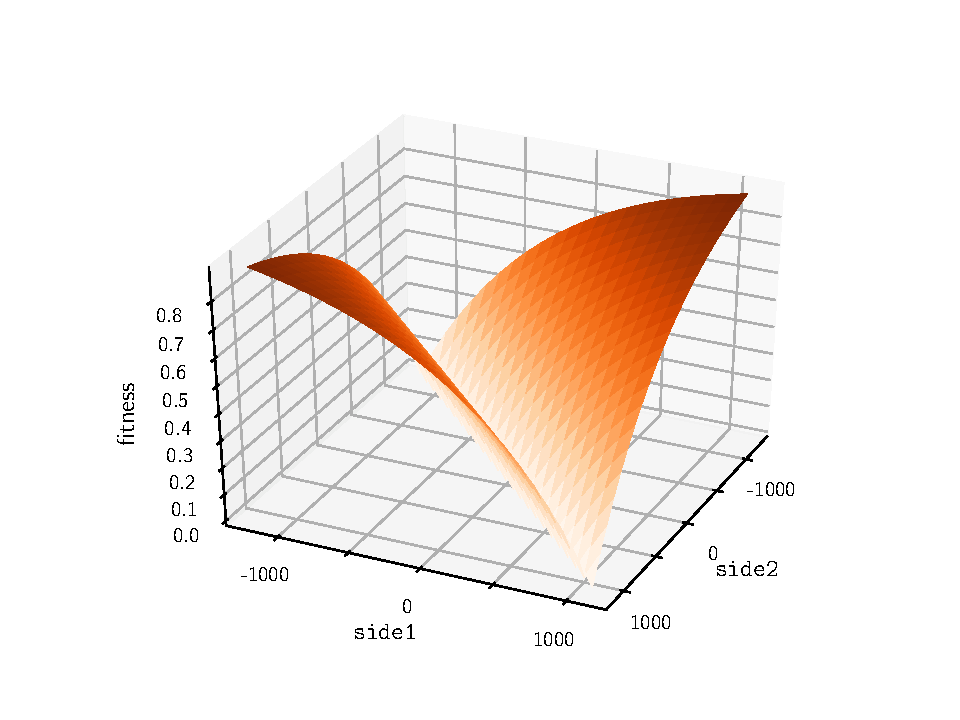
\includegraphics[width=11cm]{plots/sbst-side1-equals-side2.pdf}
    \vspace{-1em}
\end{center}

Notice that in this fitness landscape, there is a clear gradient from every
point in the input domain to the ``valley'' where the required inputs lie (i.e.,
the line where {\tt side1} equals {\tt side2}). 

Compare this to what Random Testing ``sees'': 

\begin{center}
    \vspace{-1em}
    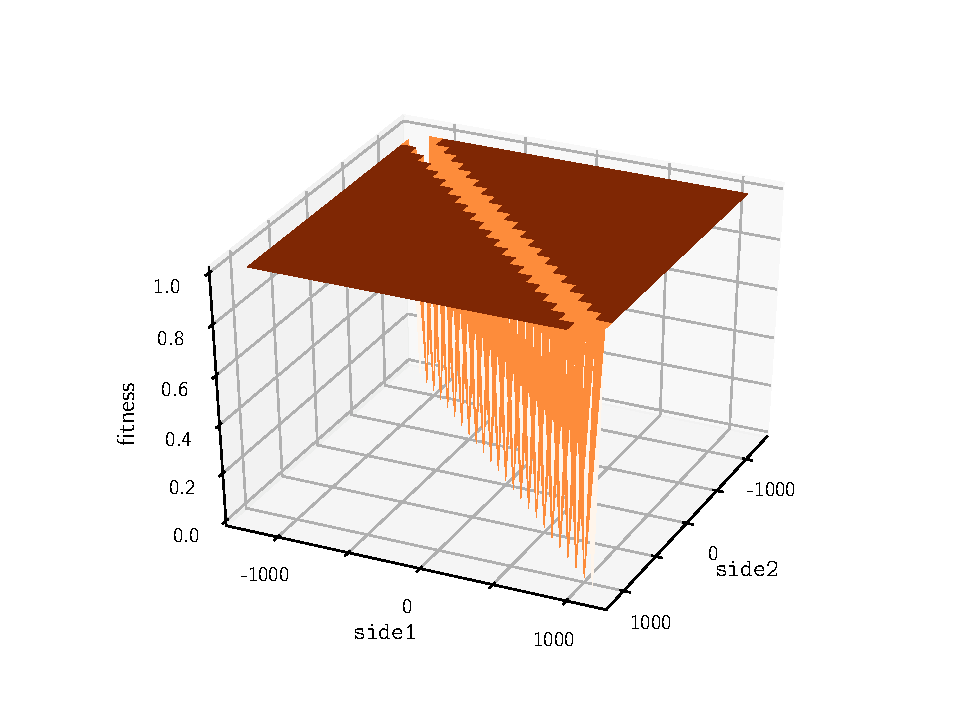
\includegraphics[width=11cm]{plots/rt-side1-equals-side2.pdf}
    \vspace{-1em}
\end{center}

Random Testing is not guided by any information, so every input is treated the
same, unless it executes the branch in question. Statistically speaking, Random
Testing will spend most of its time exploring the plateaus either side of the
valley, since there is no impetus to incrementally move towards values of {\tt
side1} and {\tt side2} that are closer together.

\section{Search Techniques}

It's all very well and good having guidance, but we need a method of exploiting
it. That's where the ``search'' part of Search-Based Testing comes in ---
Search-Based Testing uses the fitness function in combination with an
optimisation algorithm. 

\subsection{Simple Gradient Descent}

One of the simplest optimisation algorithms is a search technique called {\it
Gradient Descent}. Gradient Descent aims to travel down the gradient of the
fitness landscape to the nearest minimum. It works as follows:

\begin{enumerate}
    \item Pick a point $p$ at random in the search space (the input domain), and
    evaluate its fitness, $\mathit{fitness}(p)$.

    \item Evaluate all the neighbouring points in the fitness landscape, $p_1
    \dots p_n$.

    \item If $\mathit{fitness}(p_i), 1 < i < n$ is less than than
    $\mathit{fitness}(p)$, set $p$ to $p_i$.

    \item Jump to step 2 and repeat until none of $p_1 \dots p_n$ offer an
    improved fitness over $p$.
\end{enumerate}

Gradient Descent (often called {\it Hill Climbing} if the fitness function is to
be maximised) is often described as a ``local'' search algorithm, because as
each point, it evaluates all of its neighbours for a position of improved
fitness in the landscape, until it cannot improve fitness any more. That is, it
has reached a local minima in the fitness landscape. If this local minima
represents a fitness value of zero, the test requirement will have been
satisfied (i.e., the problematic branch is executed with the input in our
triangle example). If not, the search cannot make any more progress from this
position, so it is {\it restarted} from a different random position in the
search space, in the hope of ending up in local minimum that does satisfy the
test requirement. This process continues until the test requirement is satisfied
or some resource limit (e.g., number of iterations or test data evaluations) is
exhausted. The search will always fail, for example, if the test requirement is
infeasible. 

\subsection{The Alternating Variable Method (AVM)}

The Alternating Variable Method (AVM) is an advanced Gradient Descent algorithm
designed for generating numerical inputs for test cases quickly. The AVM is
faster than normal Gradient Descent, because, when given the opportunity, it
accelerates down a gradient rather than inching down it, step-by-step. 

The AVM alternates between small ``exploratory'' moves in the search space to
establish the direction of the gradient, and then makes ``pattern'' moves of
increasing step size in the direction of fitness improvement. 

It does this by starting with a random set of inputs, as with Gradient Descent.
It then considers each input variable in turn, increasing it by a small amount
and decreasing it (exploratory moves) --- e.g., +1 and -1 for an input of
integer type. If one of the two moves leads to an improvement in fitness, a
larger increase/decrease (a pattern move) is made (e.g., +2 or -2). If the
fitness continues to improve, the step size is continually doubled until fitness
gets worse. At this point, further exploratory moves are made to re-establish a
new ``direction'' of improved fitness. This exploratory/pattern move cycle
continues until both exploratory moves result in a non-improvement in fitness.
The AVM then moves onto the next variable and repeats the same steps. This
continues until the AVM has made a complete sweep of the input variables and
there are no exploratory improvements --- or, inputs have been found that
satisfy the test requirement.

\subsection{Evolutionary Algorithms}

Local search only samples one point in the search space (input space) at a time.
Evolutionary Algorithms are so-called ``population''-based approaches that
sample multiple points in the search space at once. In Evolutionary
Algorithm-speak, each point in the search space (i.e., an input to the program,
in this problem domain) is an ``individual''. The idea is that the good parts of
one individual can be combined with another to reach a solution to the problem. 

For example, suppose we have a branch in our program that is executed when a
inputted string contains digits only. However, strings generated purely at
random may contain any character. Strings with one or two digits initially
receive a good fitness value compared to others in the population. Evolutionary
Algorithms emphasis a search operator called ``recombination'', which involves
combining the parts of one individual with another to make an ``offspring''
individual. So a string with digits early in the string may be recombined with a
string with digits later in the string, to produce a new string with digits at
the start and the end, with an even better fitness value. 

% TODO Diagram of crossover --- from slide 

Evolutionary Algorithms also employ another search operator called ``mutation''
that makes random changes to individuals. So for a test case, this may mean
changing one the inputs to a completely new value, or changing it by some delta
value. 

% TODO Diagram of mutation --- from slide

% TODO -- complete description of EAs

% TODO Diagram of an EA --- from slide

\section{More on Fitness Functions}

For testing branch predicates beyond equality (i.e., {\tt a == b} in the table),
researchers have developed the following series of fitness functions. The term
$K$ represents a small, positive value.

\begin{center}
    \begin{tabular}{ll}
        \toprule
        {\bf Condition Type} & {\bf Fitness Function} \\
        \midrule
        {\tt a == b} & if $|${\tt a} $-$ {\tt b}$| = 0$ then $0$ else $|${\tt a} $-$ {\tt b}$| + K$ \\
        {\tt a != b} & if $|${\tt a} $-$ {\tt b}$| \neq 0$ then $0$ else $K$ \\
        {\tt a < b}  & if {\tt a} $-$ {\tt b} $< 0$ then $0$ else {\tt a} $-$ {\tt b} $+$ $K$ \\
        {\tt a <= b} & if {\tt a} $-$ {\tt b} $\leq 0$ then $0$ else {\tt a} $-$ {\tt b} $+$ $K$ \\
        {\tt a > b}  & if {\tt b} $-$ {\tt a} $< 0$ then $0$ else {\tt b} $-$ {\tt a} $+$ $K$ \\
        {\tt a >= b} & if {\tt b} $-$ {\tt a} $\leq 0$ then $0$ else {\tt b} $-$ {\tt a} $+$ $K$ \\
        \bottomrule
    \end{tabular}
\end{center}    
    
One problem with using fitness function based on the predicates in branches only
is that the branch needs to be actually {\it reached} in the code for the
fitness to be calculated. Otherwise, inputs will get the same, poor fitness
value. If the branch is hard to reach (e.g., because some other branch in the
program needs to be taken that is only executed by only a few inputs), the
search does not get any guidance and behaves more like Random Testing.

To get around this problem, the fitness function needs to care about all of the
branch predicates that need to be executed leading up to the ``target'' branch,
not just the target itself. To figure out which branches are important, we need
to go back to the concept of control flow graphs (CFGs). 

A node of a CFG (which we'll refer to as the ``execution target'') is said to be
{\it control dependent} on a branch predicate in the CFG if that branch
predicate needs to be executed in a certain way (i.e., evaluated as either true
or false) for the execution target to be reached in the program. 

Recall, the \classifymethod~method of the \triangleclass~class. Suppose node~24
is the test generation target. Node~24 is control dependent on the branch
predicate of node~20. Unless the predicate evaluates to false, node~24 will
never be reached. Furthermore, node~25 is control dependent on the branch
predicate of node~24. If the branch predicate at node~24 evaluates to false,
node~25 will not be reached by any execution path. To further understand control
dependence, note the CFG nodes that {\it do not} have control dependencies. For
example, node~20 is {\it not} control dependent on the outcome at node~14, it will
always be executed. All paths reach node~20. 

% TODO Add in slide for the Triangle program (from Symbolic Execution)

In well-structured programs, control dependencies are more or less obvious from its nesting
structure. However, when programs deploy language constructs like {\tt break},
{\tt goto} or multiple {\tt return} statements, control dependencies are not as
easy to figure out, and more complex algorithms are needed. This will be
covered in a later lecture, on the subject of {\it Program Slicing}. For now,
however, we just need to understand the general concept. 

Using the concept of control dependency, we can now assign a fitness score to
inputs based on how close they were to reaching the target branch. This fitness
score is called the {\it approach level}. For example:

Suppose the execution target of the \classifymethod~method is node~26. Node~26
is control dependent on the branch predicate of node~25, which is control
dependent on the branch predicate of node~24, which in turn is control dependent
on the branch predicate of node~20 --- three levels of control dependency.
Inputs that take the path that takes the true branch at node~20, thereby missing
nodes~24 and~25 are assigned an approach level of {\bf 2}. Inputs that take the
false branch at node~20, reaching node~24, but then evaluating the branch
predicate at node~24 as false, thereby missing node~25 are assigned an approach
level of~{\bf 1}. Finally, all inputs that take the path reaching the final
branch predicate in the control dependence chain, node~26, receive the lowest
(i.e., best, in this context) approach level of {\bf 0}.

% TODO diagram 

At each approach level, we can add the fitness for the predicate. We refer to
this part as the {\it branch distance}. The branch distance is normalised
(i.e., set to a value between 0 and 1) so that it never exceeds the approach
level component of the fitness function for that particular branching statement.

% TODO: fitness function and program 
% TODO: the usual diagram of combining branch predicate with approach level.

(There are various formulas that can achieve this normalisation without an
explicit upper bound, one being $\frac{d}{d+1}$, where $d$ is the value to be
normalised.)

\section{Other Applications of Search-Based Testing and Optimisation Algorithms
in Testing}

As well as being applied to automatically obtain structural coverage,
Search-Based Testing has been applied to other types of test requirement.

\subsection{Real-Time Systems}

One such application area is that of real-time systems, such as controller
software in embedded systems, such as those installed into cars. Often the
actions performed by these controllers are time-sensitive --- they have to
complete by a certain time period, else there are disastrous consequences. Take
for example an airbag controller. If the software fails to recognise the
conditions in which an airbag should be released, and do this in time, the
driver is placed at risk of a serious injury. 

When testing time limits, engineers are often concerned with finding its
worst-case execution time (WCET). That is, what conditions lead to the software
taking the {\it longest} period of time to execute. If the WCET exceeds an
acceptable threshold, then its back to the drawing board...

Yet, finding the WCET of a piece of software is not a straightforward task, when
you consider that it's not just about the steps programmed into the software
itself, but also the hardware it is run on, including the caching and pipelining
behaviour of the processor. 

Search-Based Testing is an ideal technique for this problem, however. Instead of
the fitness function rewarding inputs on the basis of how close they come to
executing branches, it instead rewards inputs on the basis of the time they make
the software run for. In doing this, the search can navigate a potentially large
input space to find inputs that produce some long execution times in scenarios
that engineers may not have thought of or conceived could happen.

\subsection{Functional Safety}

Search-Based Testing has also been applied to testing functional properties
about software (similar to property-based testing, but on a system level). It
has been used to simulate automated parking controllers. 

Some of these plots show simulated car positions and parking spaces, produced
from a simulated parking controller test at the car company Daimler. The fitness
function simply measured and rewarded test cases with the smallest distance to a
collision during as simulated ``park''. The first generation of the Evolutionary
Algorithm, the randomly generated parking scenarios were easy for the controller
to handle. However, as the Evolutionary Algorithm progressed, it was able to
develop trickier scenarios that eventually produced a collision, i.e., a test
failure.

% TODO: include pictures used in previous slides

\subsection{Beyond Test Case Generation}

Optimisation algorithms such as Gradient Descent and Evolutionary Algorithms
have been applied to more in software testing than just test case generation.
They have also been applied to two problems known as ``Test Suite Minimisation''
and ``Test Suite Prioritisation''. Both problems stem from very large test
suites, with too many test cases to run, because doing so would take an
inordinate amount of time. The question is, which test cases to actually
execute. Optimisation algorithms can be used to produce smaller test suites from
the original whole, or be used to produce a running order of test cases whereby
the most important are run first. These topics are the subject of a later
lecture in this module!

\section{Tools for Search-Based Testing}

You might want to check out the following Search-Based Testing tools:

\begin{itemize}

    \item {\bf EvoSuite} (\url{https://www.evosuite.org/}) is a Search-Based
    Testing tool for Java. The latest version supports up to Java 11.

    \item {\bf IGUANA} (\url{http://iguanatool.org}) is a Search-Based Test Data
    Generation tool for branch coverage of C programs. It is written in Java,
    but will only run on Java 7.

    \item {\bf The AVM Framework (AVMf)} (\url{http://avmframework.org}) is a
    Java implementation of the AVM and is an API for using the AVM for search
    problems. The GitHub repository includes examples, include one of test data
    generation for the triangle classification problem.

\end{itemize}

\end{document}